\documentclass[10pt]{article}
\usepackage[utf8]{inputenc}
\usepackage[T1]{fontenc}
\usepackage{amsmath}
\usepackage{amsfonts}
\usepackage{amssymb}
\usepackage[version=4]{mhchem}
\usepackage{stmaryrd}
\usepackage{graphicx}
\usepackage[export]{adjustbox}
\graphicspath{ {./images/} }
\usepackage{hyperref}
\hypersetup{colorlinks=true, linkcolor=blue, filecolor=magenta, urlcolor=cyan,}
\urlstyle{same}

\title{PS1a: Linear Feedback Shift Register }


\author{Due: Monday, February 5, 11:59pm}
\date{}


\begin{document}
\maketitle
In this assignment, you will write a program that produces pseudo-random bits by simulating a linear feedback shift register. In part (b), you will use it to implement a simple form of encryption for digital pictures.

For this portion of the assignment, you will:

\begin{itemize}
  \item Implement the FibLFSR class
  \item Implement unit tests using the Boost test framework
\end{itemize}

Average time to complete assignment: $\sim 5$ hours.

\section*{1 What is an LFSR?}
A linear feedback shift register (LFSR) is a register that takes a linear function of a previous state as an input. Most commonly, this function is a Boolean exclusive-or (XOR). LFSR performs discrete step operators that

\begin{itemize}
  \item Shifts the bits one position to the left
  \item Replaces the vacated bit by the bit previously at given tap positions in the register.
\end{itemize}

In general, a LFSR has three parameters that characterize the sequence of bits it produces: the number of bits $n$, the initial seed (the sequence of bits that initializes the register), and the set of tap positions tap. Figure 1) 1llustrates one step of an 11-bit LFSR with initial seed 01101000010 and tap position 8 .

\begin{center}
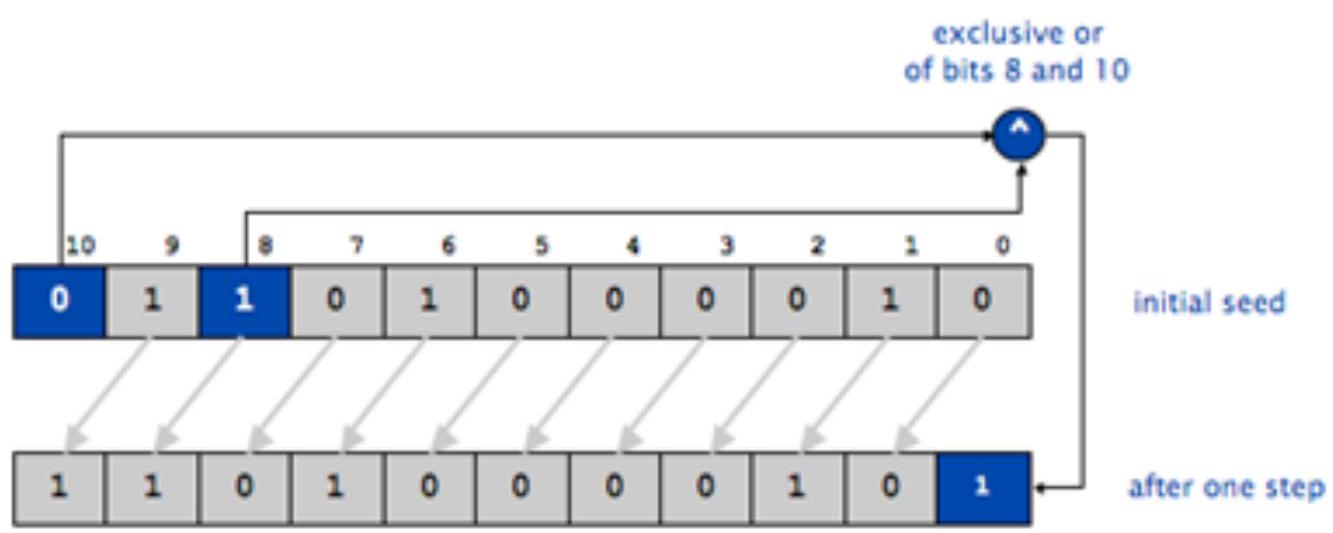
\includegraphics[max width=\textwidth]{2024_03_21_ddd7c97e7fb9b272aea0g-1}
\end{center}

One step of an 11-bit LFSR with initial seed 01101000010 and tap at position 8

Figure 1: A LFSR with a single tap at position 8. Note that position 0 is on the right side.

For this assignment, you will implement a Fibonacci LFSR which has 3 taps:

\section*{2 Fibonacci LFSR Data Type}
Your first task is to write a data type that simulates the operation of a 16-bit Fibonacci LFSR by implementing the following API:

\begin{center}
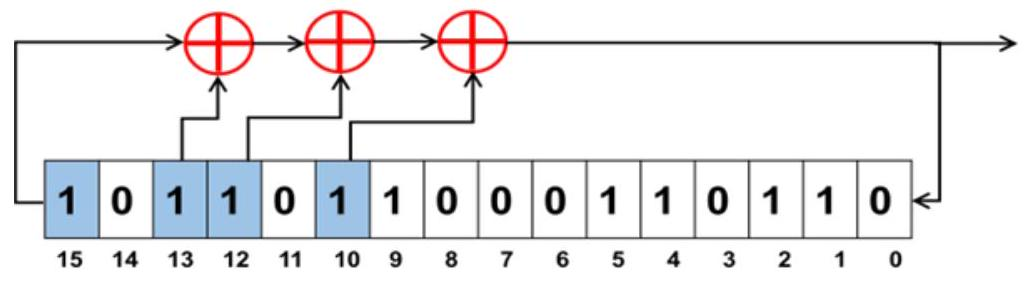
\includegraphics[max width=\textwidth]{2024_03_21_ddd7c97e7fb9b272aea0g-2}
\end{center}

Figure 2: A LFSR with taps at positions 10, 12, and 13.

\begin{center}
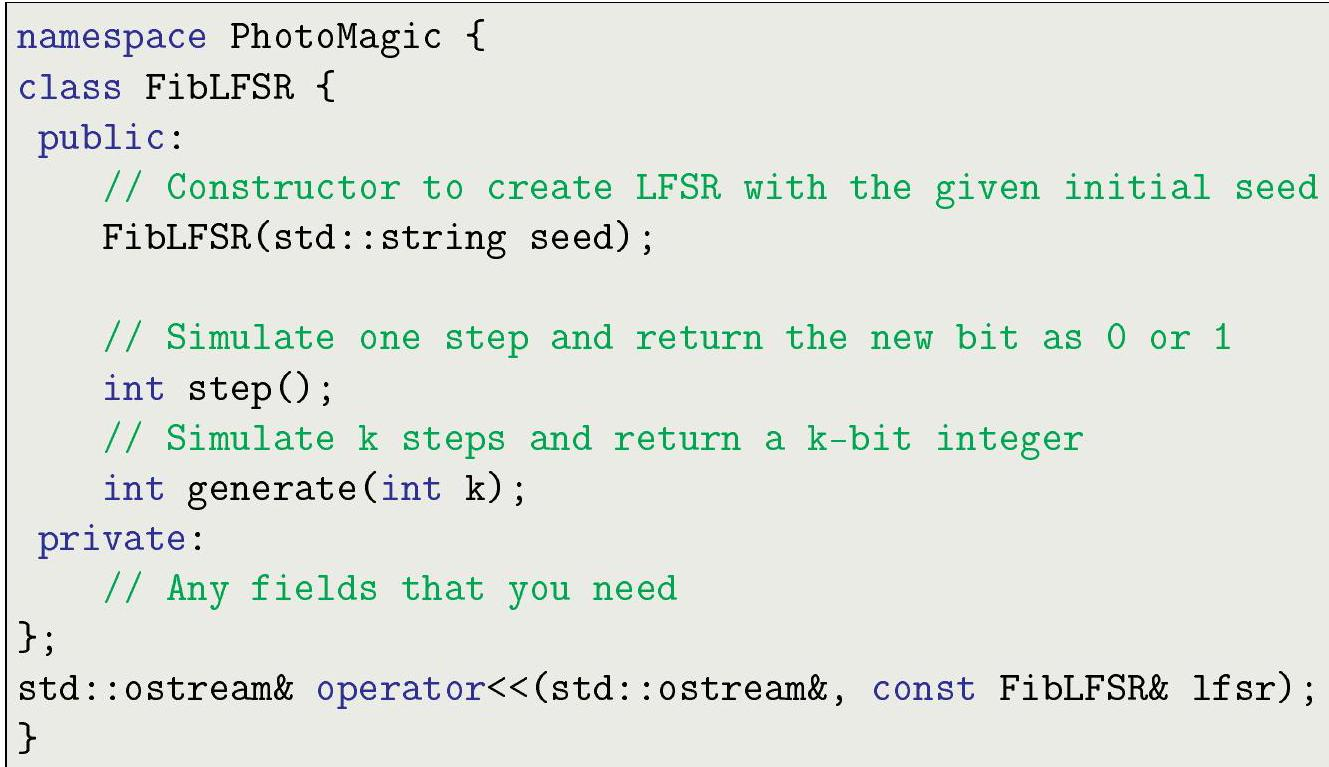
\includegraphics[max width=\textwidth]{2024_03_21_ddd7c97e7fb9b272aea0g-2(1)}
\end{center}

To do so, you will need to choose the internal representation (data fields), implement the constructor and implement the two methods and the operator. In this and future assignments, you may add additional methods and fields, but you must supply the ones listed above. These are interrelated activities and there are several viable approaches.

\section*{Constructor}
The constructor takes the initial seed as a String whose characters are a sequence of 0s and 1s. The length of the register is the length of the seed. We will generate each new bit by XORing the leftmost bit and the tap bits (using the resulting bit as one of the inputs for the next XOR operation, and so on). There are 3 taps for this assignment in positions 13, 12, and 10 (see Figure 2). For example, the following code should create the FibLFSR described above.

The FibLFSR class and any other classes or functions you write will be a part of the PhotoMagic namespace. You will add a transform function to this namespace in part $B$ and use this to build the PhotoMagic program.

FibLFSR flfsr("1011011000110110");

\section*{Destructor}
If your constructor dynamically allocates memory (with new), make sure that you define a destructor that deallocates it.

\section*{String representation}
Overload the «stream insertion operator to display its current register value in printable form. See the instructions at \href{http://www.learncpp.com/cpp-tutorial/93-overloading-the-io-operators/}{http://www.learncpp.com/cpp-tutorial/93-overloading-the-io-operators/}.

\section*{Simulate one step}
The $\operatorname{step}($ ) function simulates one step of the LFSR and returns the new rightmost bit as an integer ( 0 or 1$)$. For example, if you call step( $) 10$ times, the new state and result of each call should be:

\begin{center}
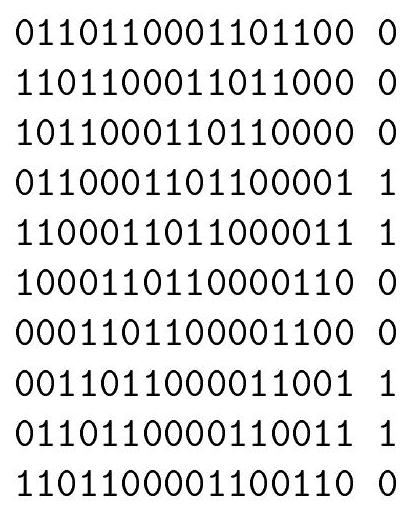
\includegraphics[max width=\textwidth]{2024_03_21_ddd7c97e7fb9b272aea0g-3}
\end{center}

\section*{Extracting multiple bits}
The member function generate() takes an integer $k$ as an argument and returns a $k$ bit integer simulating $k$ steps of the LFSR. This task is easy to accomplish with a little arithmetic: initialize a variable to zero and for each bit extracted, double the variable and add the bit returned by step(). For example, if the first 5 bits extracted are 0 , then 0 , then 0 , then 1 , then 1 , the result would be the bit sequence 00011 which corresponds to the number 3. For example, calling generate(5) seven times would give the following new states and the resulting numbers:

\begin{center}
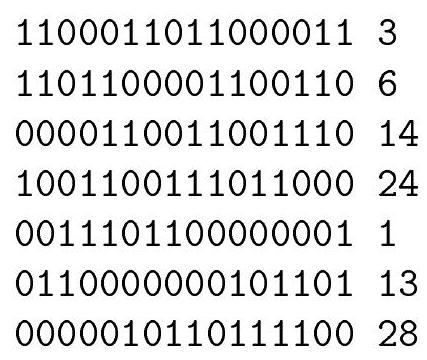
\includegraphics[max width=\textwidth]{2024_03_21_ddd7c97e7fb9b272aea0g-3(1)}
\end{center}

Implement the generate() function by calling the step() function $k$ times and performing the necessary arithmetic.

\section*{Testing}
You should have installed the Boost test framework in ps0 during the initial setup. If you didn't, do that now. You will need to link to the boost\_unit\_test\_framework library.

Use the test.cpp and add at least four unit tests using the Boost test framework (not counting the provided example tests). See \href{https://www.boost.org/doc/libs/1_53_0/}{https://www.boost.org/doc/libs/1\_53\_0/} libs/test/doc/html/utf/tutorials.html for an introduction to using Boost unit testing.

\section*{Static Libraries}
You will also create a static library file, PhotoMagic.a. This will allow the autograder to link against your library without knowing exactly which files you are submitting. This is important if you add extra .cpp files with utility functions.

You can use the ar utility to create this static library. As an example,

ar rcs PhotoMagic.a FibLFSR.o PhotoMagic.o

would create a library named PhotoMagic.a containing the code from FibLFSR.o and PhotoMagic.o.

Note that main() functions should not be included in this library. This means that your main.cpp and test.cpp files should not be included in the library (but your other .cpp files should be).

\section*{3 What to turn in}
Your makefile should build two programs, PhotoMagic and test, as well as a static library PhotoMagic.a. Your test program will run the unit tests you created and PhotoMagic will run whatever main function you created (or the tests if you didn't create one). For part (a), the behavior of progname is unspecified (in part (b) it will perform an image transform).

Submit a zip archive to Gradescope containing:

\begin{itemize}
  \item Your implementation must be contained in two files named FibLFSR . cpp and FibLFSR. hpp.
  \item The supplied test.cpp to which you added your own tests.
  \item The makefile for your project. The makefile should have targets all, PhotoMagic, test and clean. Make sure that all prerequisites are correct.
  \item Your \href{http://Readme-ps1a.md}{Readme-ps1a.md} that includes
\end{itemize}

\begin{enumerate}
  \item Your name

  \item An explanation of the representation you used for the register bits (how it works and why you selected it)

  \item A discussion of what's being tested in your four additional Boost unit tests.

\end{enumerate}

\begin{itemize}
  \item Any other source files that you created (such as main.cpp).
\end{itemize}

Make sure that all of your files are in a directory named ps1a before archiving it and that there are no .o or other compiled files in it.

\section*{4 Grading rubric}
\begin{center}
\begin{tabular}{|l|c|l|}
\hline
Feature & Points & Comment \\
\hline
Submission & 4 &  \\
\hline
 & 2 & Submits required files \\
\hline
Tests & 2 & \begin{tabular}{l}
Has targets PhotoMagic, PhotoMagic.a, test, all, and \\
clean and builds \\
\end{tabular} \\
\hline
 & 4 &  \\
\hline
 & 2 & Has at least 4 tests and passes them \\
\hline
Core Implementation & 32 & Full \& Correct Implementation \\
\hline
 & 8 & step( ) \\
\hline
 & 8 & generate () \\
\hline
 & 4 & Insertion Operator \\
\hline
 & 8 & Composite \\
\hline
Readme & 5 & Complete \\
\hline
 & 3 & \begin{tabular}{l}
Explains how the data is stored and why this representa- \\
tion was chosen \\
\end{tabular} \\
\hline
 & 2 & Explains what aspects the tests cover. \\
\hline
Penalties &  &  \\
\hline
 & -2 & Submission includes . o or . a files \\
\hline
 & -3 & Non-const global variables or public fields \\
\hline
 & -5 & Memory leaks \\
\hline
 & -5 & Linting problems \\
\hline
Total & $-10 \%$ & Each day late \\
\hline
 & 45 &  \\
\hline
\end{tabular}
\end{center}


\end{document}